%Auteurs : Nicolas Englebert
\documentclass[british,french,11pt, a4paper, openany]{book}

% Règles de bonne pratiques :
% https://fr.wikibooks.org/wiki/LaTeX/Gestion_des_gros_documents

%%%%%%%%%%%%%%%%
%%% Packages %%%
%%%%%%%%%%%%%%%%

%%% Compatibilité %%%
\begingroup\expandafter\expandafter\expandafter\endgroup
\expandafter\ifx\csname IncludeInRelease\endcsname\relax
\usepackage{fixltx2e}
\fi 					% Si version LaTeX < 2015, inclut un fix.

%%% Général %%%
\usepackage[utf8]{inputenc}
\usepackage{babel}
\usepackage{lmodern}
\usepackage[T1]{fontenc}
\addto\extrasfrench{\sisetup{locale = FR,detect-all}} % Switch siunitx en fonction de la langue babel :)
\addto\extrasbritish{\sisetup{locale = UK,detect-all}}
\usepackage{courier}
\usepackage{graphicx}
%\usepackage{cancel}

%%% Tableau %%%
%\usepackage{tabularx} %Permet d'auto dimensionner les tableaux



%%% Bibliographie %%%
%\usepackage[style=alphabetic,backend=biber]{biblatex}
\usepackage[autostyle]{csquotes}
%\DeclareNameAlias{sortname}{last-first}
%\DeclareFieldFormat{url}{\space\url{#1}}
%\DeclareNameAlias{labelname}{last-first}
%\addbibresource{sample.bib}


%%% Graphiques %%%
%\usepackage{tikz}
%\usepackage{pgfplots}
%\usepackage{circuitikz}

%%% Mise en page %%%
\usepackage{mathtools}
\usepackage{amssymb}
\usepackage{bbm}
\usepackage{amsthm}
%\usepackage[tt]{titlepic}% Centre le titre
%\usepackage{fancyhdr}   % Permet de modifier l'entête & footer
\usepackage{caption}     % Permet d'ajouter des légendes en images sans les mettre en float + dans la marge + ref vers le haut de l'envirronement
\usepackage{wrapfig}
\usepackage{fullpage}
%\usepackage{multicol}   % pour les liste sur plusieurs colonnes
%\usepackage{subfigure}  % alligne deux images cote a cote
\usepackage{float}      %permet de mettre du texte entre les figures grace a [H]. Génial! 
\usepackage{eso-pic}    % Fond d'écran page de garde
\usepackage{adjustbox}  % Empêche les box de sortir de la page


%%% Math %%%
%\usepackage{delarray} % Belles matrices
\usepackage{siunitx}


%%% Codes %%%
%\usepackage{listings}
%\usepackage[final]{pdfpages} %% Inclusion fichier pdf

%% Reference
\usepackage{hyperref}
%\renewcommand*{\figureautorefname}{fig.}
%\def\appendixautorefname{annexe}
%\def\tableautorefname{tab.}
%\renewcommand*{\chapterautorefname}{ch.}
%\newcommand{\subfigureautorefname}{\figureautorefname}



%%%%%%%%%%%%%%%%%
%%% Commandes %%%
%%%%%%%%%%%%%%%%%

%%% Physique %%%
\newcommand{\cst}{\text{cst}}
\newcommand{\D}{\partial}
\newcommand{\E}{\vec E}
\newcommand{\B}{\vec B}
\newcommand{\F}{\vec F}
\newcommand{\modu}[1]{|$#1$|}

%%% Math %%%
\newcommand{\oiint}{\int\!\!\!\!\!\!\! \:\!\subset\!\!\supset\!\!\!\!\!\!\!\int}
\newcommand{\rot}{\operatorname{\vec{rot}}}
\newcommand{\divv}{\operatorname{div}}
\newcommand{\phas}[1]{\underline{#1}}
\newcommand{\RE}{\text{Re}}
\newcommand{\ft}{\overset{\mathcal{F}}{\longleftrightarrow}}
\newcommand{\lt}{\overset{\mathcal{L}}{\longleftrightarrow}}
\newcommand{\DS}{\displaystyle}
\newcommand{\Tr}{\operatorname{Tr}}



%% Box
\shorthandon{:}
\newcommand{\theor}[1]{\adjustbox{minipage=\linewidth-2\fboxsep-2\fboxrule,fbox}{\textsc{\iflanguage{british}{Theorem}{Théorème}: }#1}}
\newcommand{\defi}[1]{\adjustbox{minipage=\linewidth-2\fboxsep-2\fboxrule,fbox}{\textsc{\iflanguage{british}{Definition}{Définition}: }#1}}
\newcommand{\lemme}[1]{\adjustbox{minipage=\linewidth-2\fboxsep-2\fboxrule,fbox}{\textsc{\iflanguage{british}{Lemma}{Lemme}: }#1}}
\newcommand{\prop}[1]{\adjustbox{minipage=\linewidth-2\fboxsep-2\fboxrule,fbox}{\textsc{\iflanguage{british}{Property}{Propriété}}\\ #1}}
\newcommand{\proposition}[1]{\adjustbox{minipage=\linewidth-2\fboxsep-2\fboxrule,fbox}{\textsc{Proposition}\\#1}}
\newcommand{\cadre}[1]{\adjustbox{minipage=\linewidth-2\fboxsep-2\fboxrule,fbox}{#1}}
\newcommand{\retenir}[1]{\adjustbox{minipage=\linewidth-2\fboxsep-2\fboxrule,fbox}{\textbf{\textit{\textsc{\iflanguage{british}{To remember}{À retenir}}: }}#1}}

\newcommand{\corollaire}[1]{\bigbreak\begin{tabular}{||c}
	\begin{minipage}{\textwidth}
		\textsc{\iflanguage{british}{Corollary}{Corollaire}: } \textit{#1}
	\end{minipage}
	\end{tabular}}
\newcommand{\exemple}[1]{\bigbreak\begin{tabular}{|c}
	\begin{minipage}{\textwidth}
		\textsc{\iflanguage{british}{Example}{Exemple}: } #1
	\end{minipage}%
	\end{tabular}}%
\shorthandoff{:}
    

%\pagestyle{headings} % Titre du ch et numéro page dans l'entete
%\renewcommand{\proofname}{Démonstration}
%\addto\captionsfrench{\def\tablename{Tableau}}


%%% Background %%%
\newcommand\BackgroundPic{%
	\put(0,0){%
		\parbox[b][\paperheight]{\paperwidth}{%
			\vfill
			\centering
			\includegraphics[width=\paperwidth,height=\paperheight,%
			keepaspectratio]{../../Builder/ulb.jpg}%
			\vfill
}}}

%%% Annexes Cedu %%%
%\usepackage{calrsfs}
%\DeclareMathAlphabet{\pazocal}{OMS}{zplm}{m}{n}
\usepackage{fourier-orns}

\setlength{\parindent}{0pt} 

%%% Attributs %%%
\newcommand*{\NomduCours}[2]{\def\cours{#1}\def\memo{#2}}
\newcommand*{\annee}[2]{\def\adebut{#1}\def\afin{#2}}

\newcounter{auteurcnt}
\newcommand\addauteur[2]{%
	\stepcounter{auteurcnt}%
	\csdef{auteur\theauteurcnt}{\mbox{#1~\textsc{#2}}}}
\newcommand\getauteur[1]{%
	\csuse{auteur#1}}

\newcounter{illustrateurcnt}
\newcommand\addillustrateur[2]{%
	\stepcounter{illustrateurcnt}%
	\csdef{illustrateur\theillustrateurcnt}{\mbox{#1~\textsc{#2}}}}
\newcommand\getillustrateur[1]{%
	\csuse{illustrateur#1}}

\newcounter{rappeltheocnt}
\newcommand\addrappeltheo[2]{%
	\stepcounter{rappeltheocnt}%
	\csdef{rappeltheo\therappeltheocnt}{\mbox{#1~\textsc{#2}}}}
\newcommand\getrappeltheo[1]{%
	\csuse{rappeltheo#1}}

\newcounter{professeurcnt}
\newcommand\addprofesseur[2]{%
	\stepcounter{professeurcnt}%
	\csdef{professeur\theprofesseurcnt}{\mbox{#1~\textsc{#2}}}}
\newcommand\getprofesseur[1]{%
	\csuse{professeur#1}}

\newcounter{iter}

%Typique Phys
\usepackage{physics}
\usepackage{multicol}

% Attributs
\NomduCours{Physique atomique}{PHYS-H-405}
\addauteur{Nicolas}{Englebert}
\addprofesseur{Michel}{Godefroid}
\annee{2016}{2017}


% Document
\begin{document}
\def\equationautorefname~#1\null{%
	(#1)\null
}
\newcommand{\notes}[1]{\bigbreak\begin{tabular}{|c}
		\begin{minipage}{\textwidth}
			#1
		\end{minipage}%
\end{tabular}}%
%%%%%%%%%%%%%%%%%
% Préliminaires %
%%%%%%%%%%%%%%%%%
\frontmatter
\AddToShipoutPicture*{\BackgroundPic}

\begin{titlepage}
	\begin{center}	
			
		\newcommand{\HRule}{\rule{\linewidth}{0.5mm}}   			            %Titre en gros
		\includegraphics[width=0.55\textwidth]{../../Builder/titlepage/logo.pdf}~\\[1cm]				%Logo
			
			\textsc{\LARGE Université Libre de Bruxelles}\\[1.5cm]
			\textsc{\Large \iflanguage{british}{Summary}{Synthèse}}\\[0.5cm]
			
			\HRule \\[0.4cm]
			{ \huge \bfseries \cours \ \\\memo \\[0.4cm] }
			
			
			\HRule \\[1.5cm]
			\begin{minipage}[t]{0.6\textwidth}
				\begin{flushleft}%\large
					\emph{\iflanguage{british}{Author}{Auteur}\ifnum\theauteurcnt>1 s\fi:}\\
					\whileboolexpr
					{ test {\ifnumcomp{\value{iter}}{<}{\theauteurcnt}} }%
					{\stepcounter{iter}\getauteur{\theiter}\\}
					\setcounter{iter}{0}%
					\ifnum\theillustrateurcnt>0%
					\ \\
					\emph{Illustrations:}\\
					\whileboolexpr
					{ test {\ifnumcomp{\value{iter}}{<}{\theillustrateurcnt}} }%
					{\stepcounter{iter}\getillustrateur{\theiter}\\}%
					\setcounter{iter}{0}%
					\fi%
					\ifnum\therappeltheocnt>0%
					\ \\
					\emph{\iflanguage{british}{Reminders}{Rappels théoriques}:}\\
					\whileboolexpr
					{ test {\ifnumcomp{\value{iter}}{<}{\therappeltheocnt}} }%
					{\stepcounter{iter}\getrappeltheo{\theiter}\\}%
					\setcounter{iter}{0}%
					\fi%
				\end{flushleft}
			\end{minipage}%
			\begin{minipage}[t]{0.25\textwidth}
				%\begin{flushright}
				%\large
				\emph{\iflanguage{british}{Professor}{Professeur}\ifnum\theprofesseurcnt>1 s\fi:}
				\whileboolexpr
				{ test {\ifnumcomp{\value{iter}}{<}{\theprofesseurcnt}} }%
				{\\ \stepcounter{iter}\getprofesseur{\theiter}}%
				\setcounter{iter}{0}%
				%\end{flushright}
			\end{minipage}
			
			\vfill
			
			% Bottom of the page
			{\large \iflanguage{british}{Year}{Année} \adebut~-~\afin}
			
		\end{center}
	\end{titlepage}

\ \\[2cm]
{\Huge \bfseries Appel à contribution}\\[5mm]
\subsection*{Synthèse Open Source}
\begin{wrapfigure}[5]{l}{4.5cm}
	\includegraphics[scale=0.5]{../../Builder/git.png}
\end{wrapfigure}
Ce document est grandement inspiré de l’excellent cours donné 
par \ifnum\theprofesseurcnt=1 \getprofesseur{1} \else\whileboolexpr
{ test {\ifnumcomp{\value{iter}}{<}{\theprofesseurcnt-2}} }%
{\stepcounter{iter}\getprofesseur{\theiter}, }%
\stepcounter{iter}\getprofesseur{\theiter} et \stepcounter{iter}\getprofesseur{\theiter} \fi%
 à l’EPB (École Polytechnique de Bruxelles), faculté de l’ULB (Université 
Libre de Bruxelles). Il est écrit par les auteurs susnommés avec l’aide de tous les autres étudiants 
et votre aide est la bienvenue ! En effet, il y a toujours moyen de l’améliorer surtout que si le 
cours change, la synthèse doit être changée en conséquence. On peut retrouver le code source à l’adresse 
suivante
\begin{center}
	\url{https://github.com/nenglebert/Syntheses}
\end{center}\bigskip
Pour contribuer à cette synthèse, il vous suffira de créer un compte sur \textit{Github.com}. De
légères modifications (petites coquilles, orthographe, ...) peuvent directement être faites sur le
site ! Vous avez vu une petite faute ? Si oui, la corriger de cette façon ne prendra que quelques 
secondes, une bonne raison de le faire ! \bigskip

Pour de plus longues modifications, il est intéressant de disposer des fichiers : il vous 
faudra pour cela installer \LaTeX, mais aussi \textit{git}. Si cela pose problème, nous sommes 
évidemment ouverts à des contributeurs envoyant leur changement par mail ou n’importe quel autre 
moyen.\bigskip

Le lien donné ci-dessus contient aussi un \texttt{README} contenant de plus amples informations, 
vous êtes invités à le lire si vous voulez faire avancer ce projet ! 

\subsection*{Licence Creative Commons}
\begin{wrapfigure}[3]{r}{2.8cm}
	\vspace{-5mm}
	\includegraphics[scale=0.17]{../../Builder/CC}
\end{wrapfigure}
Le contenu de ce document est sous la licence Creative Commons : \textit{Attribution-NonCommercial-ShareAlike 
4.0 International (CC BY-NC-SA 4.0)}. Celle-ci vous autorise à l'exploiter pleinement, compte-
tenu de trois choses :
\begin{enumerate}
	\item \textit{Attribution} ; si vous utilisez/modifiez ce document vous devez signaler le(s) nom(s)
	      de(s) auteur(s).
	\item \textit{Non Commercial} ; interdiction de tirer un profit commercial de l’œuvre sans 
	      autorisation de l'auteur 
	\item \textit{Share alike} ;  partage de l’œuvre, avec obligation de rediffuser selon la même 
	      licence ou une licence similaire
\end{enumerate}
Si vous voulez en savoir plus sur cette licence :
\begin{center}
	\url{http://creativecommons.org/licenses/by-nc-sa/4.0/}
\end{center}

\begin{flushright}
	\textbf{Merci ! }
\end{flushright}
\tableofcontents
%Si abstract, \input ici

%%%%%%%%%%%%%%%%%%%%%
% Contenu principal %
%%%%%%%%%%%%%%%%%%%%%
\mainmatter
\chapter{Interaction des particules chargées avec la matière : considérations de base}
\section{Introduction}
Il existe trois types de rayonnements ionisants (\textit{ionizing radiations})
\begin{enumerate}
\item Les particules chargées
\begin{itemize}
\item Électron, positron, ions, \dots
\end{itemize}
\item Les photons (particules neutres sans masses)
	\begin{itemize}
	\item Les $\gamma$ (origine \textbf{nucléaire})
	\item Les $X$ (origine atomique)
	\end{itemize}
\item Neutrons (particules neutres)
\end{enumerate}
Notons que ce qui fait vraiment la différence entre un $\gamma$ et un $X$ est le mode 
d'émission et non pas l'énergie (conséquence).\\

Pour chacun de ces types de rayonnement, il existe un mécanisme d'interaction particulier
avec la matière\footnote{\textit{Assemblage d'atomes isolés sans interaction entre-eux : 
gaz d'atome}. Il s'agit de la définition de ce cours, qui évoluera au fil des chapitres}. 
\begin{itemize}
\item[$\bullet$] Les particules chargées interagissent par interactions coulombienne 
(noyaux et électrons), les collisions sont donc fréquentes et on peut considérer que 
l'énergie est perdue de façon (quasi-)continue. La particule s'arrête ainsi à distance 
finie dans la matière de sorte à ce qu'on puisse définir un "parcours" (\textit{range}) 
de celle ci  : de tels rayonnements sont \textit{directement} ionisants
\item[$\bullet$] Les particules neutres (pas d'interaction coulombienne) ont une 
probabilité de traverser la matière sans interactions, il n'est donc pas possible de 
définir un range. Elles peuvent par contre déposées de l'énergie à des particules 
chargées qui vont causés une ionisation : de tels rayonnements sont \textit{indirectement} 
ionisants
\end{itemize}
Les interactions d'un rayonnement avec la matière peut modifier l'état du rayonnement 
(absorbé, dévié, \dots) et aussi l'état de la matière (excités, ionisés,\dots).

\newpage
\subsection{Interaction des particules chargées avec la matière}
	\begin{wrapfigure}[7]{l}{6cm}
	\vspace{2mm}
	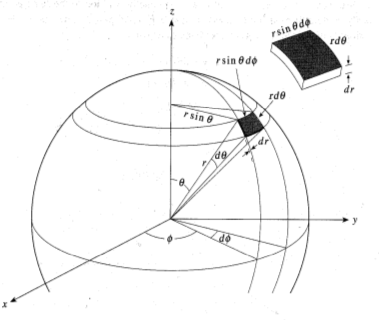
\includegraphics[scale=0.4]{ch1/image1.png}
	\captionof{figure}{Trajectoire d'une particule chargée}
	\end{wrapfigure}
Comme annoncé ci-dessus, les particules chargées subissent des collisions 
coulombiennes\footnote{Les réactions nucléaires sont laissées de côté.} avec :
\begin{description}
\item[Les noyaux (rare)] : cause une importante perte d'énergie et une grande déviation
angulaire
\item[Les électrons (fréquent)] : cause des excitations/ionisations se traduisant par des
faibles pertes d'énergie et déviations angulaires
\end{description}\ \\

	\begin{wrapfigure}[7]{r}{6cm}
	\vspace{-9mm}
	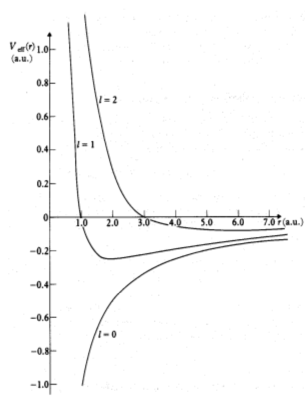
\includegraphics[scale=0.4]{ch1/image2.png}
	\captionof{figure}{ }
	\end{wrapfigure}
Chaque collision cause alors une perte d'énergie $T_j$, causés par un grand nombre de 
projectiles $N$ qui suivent $N$ histoires propres : le nombre de collision étant très 
important, les fluctuations sont faibles et il devient possible de définir des quantités
moyennes.\\

Pour introduire ces valeurs moyennes, il faut avant tout introduire la notion de 
\textbf{section efficace}.\ \\

\cadre{La \textbf{section efficace} est l'aire fictive que doit avoir une particule incidente
pour reproduire la probabilité de collision observée avec une particule cible.}\ \\

	\begin{wrapfigure}[7]{l}{6cm}
	\vspace{-5mm}
	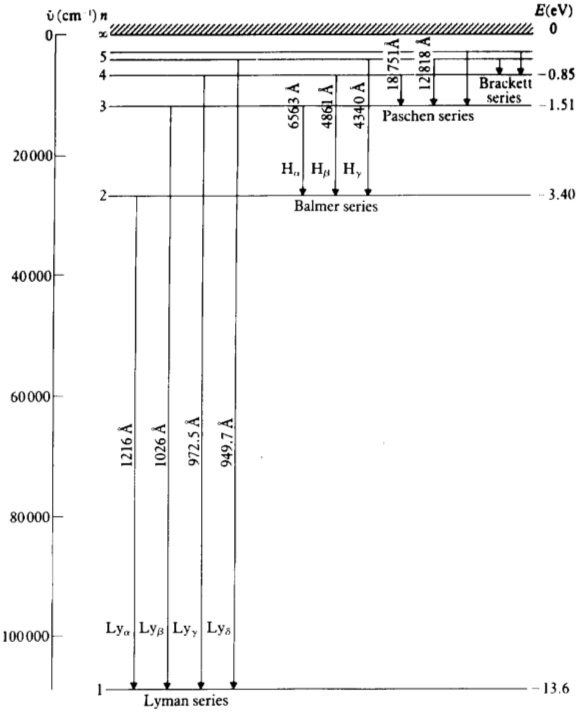
\includegraphics[scale=0.5]{ch1/image3.png}
	\captionof{figure}{ }
	\end{wrapfigure}
Il existe plusieurs sortes de section efficace. Pour s'en rendre compte, définissons ce
qu'est une collision. Il s'agit de \textit{l'interaction entre une particule incidente et une particule cible qui implique un effet spécifique mesurable}. Ainsi, la section efficace ne 
dépend pas que des particules incidentes/cibles et de leur vitesse \textbf{mais aussi} de l'effet
physique !\\
\ \\

Sur le grand nombre d'interaction existant, on peut s'intéresser à une perte d'énergie 
(section efficace différentielle en énergie $d\sigma/dE$) ou à une émission dans une 
direction donnée ((section efficace différentielle en énergie $d\sigma/d\Omega$).\\

	\begin{wrapfigure}[7]{r}{5cm}
	\vspace{-9mm}
	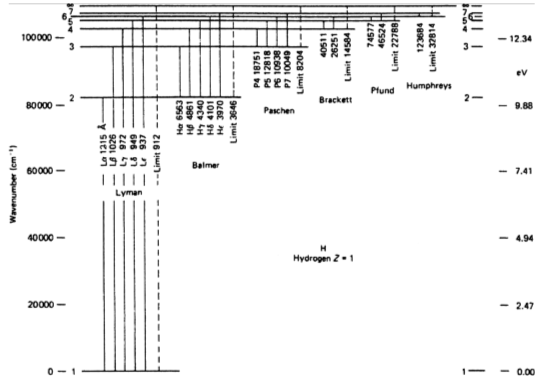
\includegraphics[scale=0.5]{ch1/image4.png}
	\captionof{figure}{ }
	\end{wrapfigure}
Quel est le rapport avec les valeurs moyennes annoncées ci-dessus ? Il n'est pas possible 
de déterminer expérimentalement les sections efficaces microscopiques en bombardant un 
atome avec une seule particule, il va falloir travailler avec des informations 
\textbf{statistiques} venant d'un bombardement (faisceau) sur la matière (milieu). Nous 
ferons l'hypothèse que les projectiles du faisceau n'interagissent pas entre-eux.\newpage

	\begin{wrapfigure}[9]{r}{4cm}
%	\vspace{-9mm}
	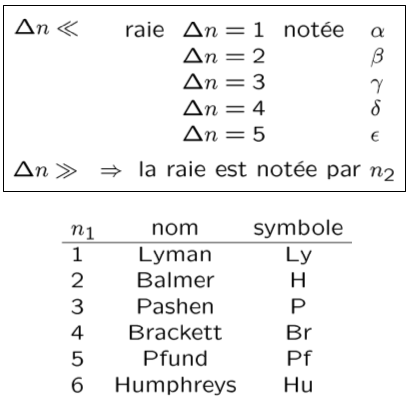
\includegraphics[scale=0.35]{ch1/image5.png}
	\captionof{figure}{ }
	\end{wrapfigure}
La section efficace sera ainsi définie par une probabilité. Soit un faisceau de particule
(densité de courant $J$), un milieu cible (aire $S$ plus petites que l'aire du faisceau)
et processus d'interaction $A$ (caractérisé par $\sigma_A$). Le nombre d'interaction $A$ 
induits par le faisceau par unité de temps $n_A$ s'écrit
\begin{equation}
n_A=JS\times\frac{\sigma_A}{S}=J\sigma_A
\end{equation}\ \\
Considérons un volume $V=S.x$ et une densité de particule cible $N$ 
\begin{equation}
n_A=N\times Sx\times J\sigma_A=JS\times Nx\sigma_A\quad\Rightarrow\quad P_A=Nx\sigma_A
 {\mbox{~~~~pour~~~~}}Nx\sigma_A\ll 1
\end{equation}
où $P_A$ est la probabilité pour un projectile de subir un processus $A$.\\

Dans le cas où $N.x.\sigma_A$ n'est pas petit, on peut observer une collision et, s'il 
n'y a pas d'absorption, la particule peut en subir une nouvelle : on parle de \textbf{
collisions multiples}. Soit $P_n$ la probabilité d'initier $n$ événements $A$. Cette 
situation est équivalente à considérer $n$ particules cibles dans un cylindre de volume 
$v=x.\sigma_A$ associé à une trajectoire. Ce problème est un classique de la théorie 
cinétique des gaz, on peut montrer que $P_n$ quit une distribution de Poisson
\begin{equation}
P_n=\frac{(Nv)^n}{n!}e^{-Nv}
\end{equation}
La valeur moyenne se définit alors comme
\begin{equation}
\langle n \rangle=Nv=Nx\sigma_A
\end{equation}
On en tire la \textsc{Loi de Lambert \& Beer} gouvernant les phénomènes d'absorption
\begin{equation}
P_0=e^{-Nx\sigma_A}
\end{equation}
Il s'agit de la probabilité de ne pas se faire absorbé. Si $Nx\sigma_A\ll 1$, on peut 
utiliser l'approximation suivante
\begin{equation}
P_n\simeq\left\{
\begin{aligned}
   &1-Nx\sigma_A& {\mbox{~~~~pour~~~~}} n=0\\
   &Nx\sigma_A& {\mbox{~~~~pour~~~~}} n=1\\
   &0&{\mbox{~~~~pour~~~~}} n\ge 2
\end{aligned} 
\right.
\end{equation}
Cette distribution nous permet de définir aisément la distance moyenne entre deux 
processus de type $A$, soit le \textbf{libre parcours moyen $\lambda_A$}
\begin{equation}
\lambda_A=\frac{1}{N\sigma_A}
\end{equation}
Ceci se généralise pour les processus multiples
\begin{equation}
\sigma_{total}=\sigma_A+\sigma_B+\sigma_C+\dots,\qquad \frac{1}{\lambda_{total}}=\frac{1}{\lambda_{A}}+\frac{1}{\lambda_{B}}+\frac{1}{\lambda_{C}}+\dots
\end{equation}


\subsubsection{Pouvoir d'arrêt}
Les pertes en énergies sont caractérisée par le \textbf{pouvoir d'arrêt} (\textit{stopping power}) : il s'agit de la grandeur la plus importante pour une particule chargée. Il s'agit - pour une 
particule chargée d'énergie cinétique $E$ dans un matériau - de la perte d'énergie moyenne
($\Delta E$) par unité de longueur subie par la particule le long de sa trajectoire ($\Delta x$)
\begin{equation}
\dfrac{\Delta E}{\Delta x}\qquad [J.M^{-1}] = [eV.m^{-1}]
\end{equation}
Afin de l'exprimer mathématiquement, considérons une cible de petite épaisseur (par rapport 
à la profondeur de pénétration) $\Delta x$ et un projectile d'énergie $E$. En considérant des 
pertes d'énergies discrète $T_j \ll E$ :
\begin{equation}
\Delta E = \sum_j n_jT_j
\end{equation}
L'énergie moyenne se calcule donc
\begin{equation}
\langle \Delta E \rangle= \sum_j \langle n_j \rangle T_j
\end{equation}
où $\langle n_j\rangle=N\Delta x\sigma_j$. Nous avons alors
\begin{equation}
\langle \Delta E \rangle = N \Delta x \sum_j T_j \sigma_j
\end{equation}
En définissant la \textbf{section efficace d'arrêt} $S$
\begin{equation}
S = \sum T_j\sigma_j
\end{equation}
On définit le \textbf{pouvoir d'arrêt}\ \\

\cadre{\begin{equation}
\frac{\langle \Delta E \rangle}{\Delta x}= NS=N\sum_j T_j \sigma_j
\end{equation}}\ \\

Le pouvoir d'arrêt est donc une propriété \textit{macroscopique} tandis que la section 
efficace d'arrêt est une propriété \textit{microscopique}.

\subsubsection{Paramètres de straggling}
Tant que nous sommes dans les statistiques, calculons les écarts quadratiques moyens des
fluctuations en énergie
\begin{equation}
\Omega^2=\overline{(\Delta E-\langle \Delta E \rangle)^2}
\end{equation}
En considérant $\Delta E-\langle \Delta E \rangle= \sum_j (n_j-\langle n_j \rangle) T_j$, 
on obtient
\begin{equation}
\overline{(\Delta E-\langle \Delta E \rangle)^2}= \sum_{j ,l}\overline{(n_j-\langle n_j \rangle) (n_l-\langle n_l \rangle)}T_jT_l
\end{equation}
Deux cas sont possibles
\begin{enumerate}
\item $j=l$; on peut utiliser les propriétés de la distribution de Poisson
\begin{equation}
\overline{(n_j-\langle n_j \rangle)^2}=\langle n_j \rangle=N\Delta x \sigma_j
\end{equation}
\item $j\neq m$; on transforme la moyenne du produit en produit des moyennes 
(ceci suggère l'indépendance statistiques des différents types de collisions)
\begin{equation}
\overline{(n_j-\langle n_j \rangle) (n_l-\langle n_l \rangle)}=\overline{(n_j-\langle n_j \rangle)}\times\overline{(n_l-\langle n_l \rangle)}
\end{equation}
Or, comme $\overline{n_j-\langle n_j \rangle}=0$, les termes avec $j\neq l$ sont nuls
\end{enumerate}
On obtient donc
\begin{equation}
\Omega^2=\sum_j\langle n_j \rangle T_j^2=N\Delta x\sum_jT_j^2\sigma_j=N\Delta xW
\end{equation}
où $W$ est le \textbf{paramètre de straggling} qui \textit{caractérise les fluctuations en 
énergie} et est défini comme\footnote{Paramètre microscopique.}\ \\

\cadre{\begin{equation}
W=\sum_j T_j^2 \sigma_j
\end{equation}}\ \\

\subsubsection{Notation intégrale et cible épaisse}
Comme annoncé, le grand nombre de collision implique une perte d'énergie quasi-continue (et 
donc un spectre continu)
\begin{equation}
\sigma_j \rightarrow \frac{d\sigma}{dT}\Delta T_j
\end{equation}
Si $\Delta T_j$ est suffisamment petit, les sommes deviennent des intégrales\ \\

\cadre{\begin{equation}
S = \int T\ d\sigma,\qquad\qquad\qquad W = \int T^2 d\sigma
\end{equation}
où $d\sigma =  \frac{d\sigma}{dT}dT$.}\ \\

Nous avions jusqu'ici considéré $\Delta x$ petit impliquant $E$ constant, mais en général $S$
et $W$ dépendent de $E$. En considérant que les fluctuations des pertes d'énergies sont 
négligeables, l'énergie $E$ est bien définie en fonction de la profondeur de pénétration 
$x$\footnote{$E\to E(x)$}. On fait alors l'\textit{approximation du ralentissement continu}
(\textit{Continuous Slowing Down Approximation} - CSDA)\ \\

\cadre{\begin{equation}
\dfrac{dE}{dx} = -NS(E)
\end{equation}
où le signe négatif tient compte de la diminution d'énergie du projectile.}\ \\

Le parcours (\textit{range}) $R$ d'une particule chargée d'énergie $E$ dans un milieu est 
la valeur moyenne $\langle l \rangle$ de la longueur $l$ de sa trajectoire suivie 
jusqu'à son arrêt (sans tenir compte du mouvement thermique). En CSDA, on trouve comme 
profondeur de pénétration
\begin{equation}
x=\int^{E}_{E(x)}\frac{dE'}{NS(E')}
\end{equation}
Le \textit{range} en CSDA est donné pour $x=l$ avec $E(l)=0$
\begin{equation}
R_{CSDA}=\int^{E}_{0}\frac{dE'}{NS(E')}
\end{equation}
Rappelons que cette expression valable pour un straggling en énergie négligeable, à cause 
de notre première hypothèse.


\subsubsection{Modèle classique du pouvoir d'arrêt}
Il s'agit d'un modèle classique non-relativiste établi en 1913 par Niels \textsc{Bohr} qui
est incroyablement correct pour une certaine plage d'énergie.\\

	\begin{wrapfigure}[7]{l}{7cm}
	\vspace{-8mm}
	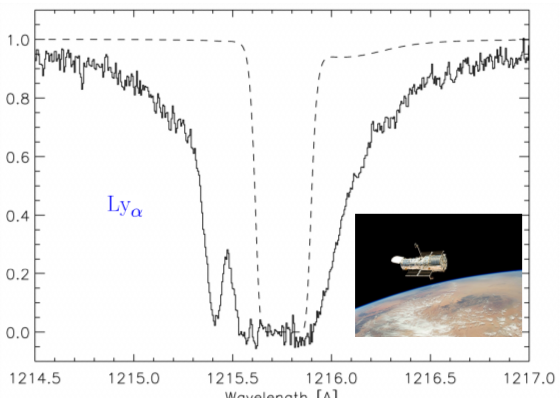
\includegraphics[scale=0.55]{ch1/image6.png}
	\captionof{figure}{ }
	\label{fig:1.6}
	\end{wrapfigure}
Soit un projectile de charge $e_1$, de masse $m_1$, de vitesse $v$ et une particule cible
($m_2,e_2$) initialement \textbf{au repos}. Cette condition initiale implique un 
\textit{scattering de Coulomb} avec un paramètre d'impact $p$\footnote{Pour rappel, il 
s'agit de la distance entre la trajectoire initiale de 1 et 2.} supposé \textit{pas trop 
petit} (\textit{soft collision}).\\

	\begin{wrapfigure}[9]{r}{6cm}
	\vspace{-8mm}
	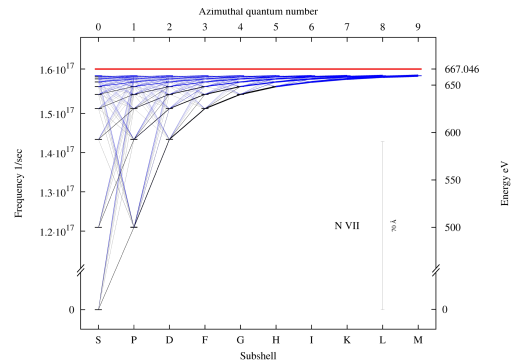
\includegraphics[scale=0.55]{ch1/image7.png}
	\captionof{figure}{ }
	\end{wrapfigure}
Supposons que la particule cible reçoit une quantité de mouvement faible tel qu'elle peut 
être considérée au repos durant l'interaction : on note le transfert de la quantité de
mouvement (unités CGS)
\begin{equation}
\overrightarrow{\Delta P}=\int_{-\infty}^{+\infty} dt \overrightarrow{F}(t)
\end{equation}
où $\DS F(t)=\frac{e_1e_2}{p^2+(vt)^2}$. En décomposant la force $\overrightarrow{F}=
F_{\parallel}\overrightarrow{1_{\parallel}}+F_{\perp}\overrightarrow{1_{\perp}}$, on 
obtient les composantes $\parallel$ et $\perp$ du transfert de quantité de mouvement\footnote{J'étais en retard\dots Quelqu'un à des notes? Sur le graphique surtout}
\begin{eqnarray}
&&\Delta P_\parallel=e_1e_2\int_{-\infty}^{+\infty}dt\frac{vt}{(p^2+(vt)^2)^{3/2}}=0\\
&&\Delta P_\perp=e_1e_2\int_{-\infty}^{+\infty}dt\frac{p}{(p^2+(vt)^2)^{3/2}}=\frac{2|e_1e_2|}{pv}
\end{eqnarray}
Il est possible d'estimer la durée de la collision, qui correspond au temps durant lequel 
le transfert d'énergie se passe
\begin{equation}
\Delta P_{\perp}\simeq F_{max}\tau
\end{equation}
où $F_{max} = e_1e_2/p^2$, la force pour la distance minimale d'approche ($p$ en $t=0$). En 
substituant, on trouve
\begin{equation}
\tau\simeq\frac{2p}{v} 
\end{equation}
Cette expression est cohérente avec la \autoref{fig:1.6} ($p/v$ à gauche et à droite, d'où le facteur 2).Il ne s'agit que d'un ordre de grandeur qui nous informe que les deux particules interagissent
de même façon effective sur une distance $2p$ le long de la trajectoire de la particule incidente.\\

	\begin{wrapfigure}[8]{l}{6cm}
	\vspace{-10mm}
	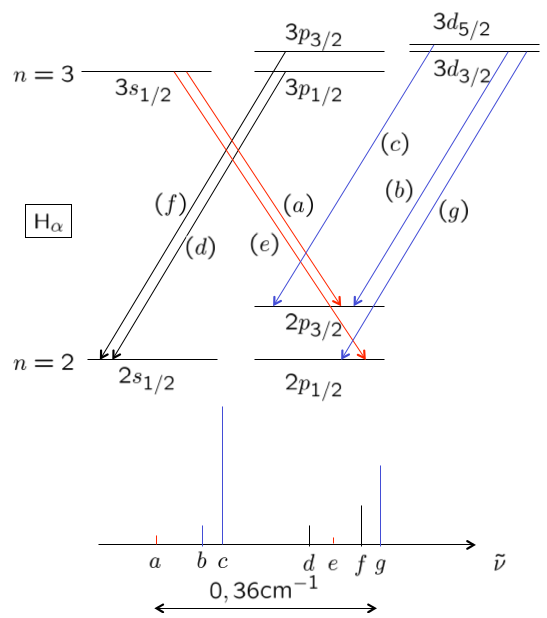
\includegraphics[scale=0.55]{ch1/image8.png}
	\captionof{figure}{ }
	\end{wrapfigure}
L'énergie $T$ transférée de 1 vers 2 s'obtient en explicitant $\Delta P_\perp^2$
\begin{equation}
T=\frac{\Delta P_\perp^2}{2m_2}\simeq \frac{2e_1^2e_2^2}{m_2v^2p^2}
\label{eq:1.ad}
\end{equation}
Le seul paramètre (aléatoire) dont dépend $T$ est le paramètre d'impact $p$. Ainsi, le nombre
de collisions caractérisés par un transfert d'énergie compris entre $T$ et $T+dT$ est caractérisé
par un paramètre d'impact entre $p$ et $p+dp$. Comme nous sommes en présence d'une géométrie
cylindrique, la particule incidente devra se trouver dans un anneau. La section efficace du 
projectile $d\sigma$ doit forcément être l'aire de cet anneau
\begin{equation}
d\sigma=2\pi pdp=\left|\frac{d(\pi p^2)}{dT}\right| dT
\label{eq:1.se}
\end{equation}
En calculant la dérivée de \eqref{eq:1.ad} dans l'expression \eqref{eq:1.se}, on trouve 
la forme de la section efficace de Rutherford pour la diffusion (scattering) coulombienne qui 
sera déduite bien plus tard (exactement) par la mécanique quantique.\ \\

\cadre{\begin{equation}
d\sigma \approx 2\pi\dfrac{e_1^2e_2^2}{m_2v^2}\dfrac{dT}{T^2}
\end{equation}}\ \\

\subsubsection{Résultats préliminaires}
Cette formule nous permet d'obtenir des résultats préliminaire pour le stopping et le 
straggling. Sachant que $S = \int Td\sigma$ et $W = \int T^2d\sigma$, on trouve
\begin{equation}
S\simeq 2\pi \frac{e_1^2e_2^2}{m_2v^2}\int_{T_{max}}^{T_{min}}\frac{dT}{T},\qquad\qquad
W\simeq 2\pi \frac{e_1^2e_2^2}{m_2v^2} \int_{T_{max}}^{T_{min}}dT
\end{equation}
Après intégration (à connaitre \textbf{par coeur}!)\ \\

\cadre{
\begin{eqnarray}
&&S\simeq 2\pi \frac{e_1^2e_2^2}{m_2v^2}\int_{T_{max}}^{T_{min}}\frac{dT}{T}\vspace{2mm}\\
&&W\simeq 2\pi \frac{e_1^2e_2^2}{m_2v^2} \int_{T_{max}}^{T_{min}}dT
\end{eqnarray}}\ \\

En utilisant le \textbf{nombre d'arrêt} (\textit{stopping number}) $\DS 
L=\frac{1}{2}\ln{\left(\frac{T_{max}}{T_{min}}\right)}$ on peut ré-écrire
\begin{equation}
S\simeq 4\pi \frac{e_1^2e_2^2}{m_2v^2}L
\end{equation}

\textsc{Résultats préliminaires pour le stopping}\ \\
Soit les électrons $(e)$ de la cible (densité $NZ_2$, masse $m$ et charge $-e$) et les 
noyaux $(n)$ de la cible (densité $N$, masse $M_2$ et charge $Z_2e$). On peut calculer 
l'énergie moyenne en multipliant $S_e$ par $NZ_2\Delta x$. En faisant de même pour $S_n$ :
\begin{eqnarray}
&&S_e=\frac{4\pi e_1^2e^2}{mv^2}L_e \Rightarrow  \langle \Delta E\rangle_e\simeq NZ_2\Delta x \times \frac{4\pi e_1^2e^2}{mv^2}L_e\vspace{2mm}\\
&&S_n=\frac{4\pi e_1^2Z_2^2e^2}{M_2v^2}L_n \Rightarrow  \langle \Delta E\rangle_n\simeq N\Delta x \times \frac{4\pi e_1^2Z_2^2e^2}{M_2v^2}L_n
\end{eqnarray}
Effectuons le rapport de ces deux dernières expressions
\begin{equation}
\frac{\langle \Delta E\rangle_n}{\langle \Delta E\rangle_e}\simeq \frac{m}{M_2}Z_2\frac{L_n}{L_e}
 {\mbox{~~or~~}} \frac{mZ_2}{M_2}<10^{-3}
\end{equation}
En laissant pour l'instant tomber le rapport des $L$ (straggling number), on obtient un terme 
inférieur à $10^{-3}$ : un électron incident va perdre beaucoup plus d'énergie lorsqu'il va 
interagir avec d'autres électrons plutôt qu'avec des neutrons.

\newpage
\subsubsection{Détermination de l'énergie transférée maximale $T_{max}$}
	\begin{wrapfigure}[8]{r}{3.5cm}
	\vspace{-5mm}
	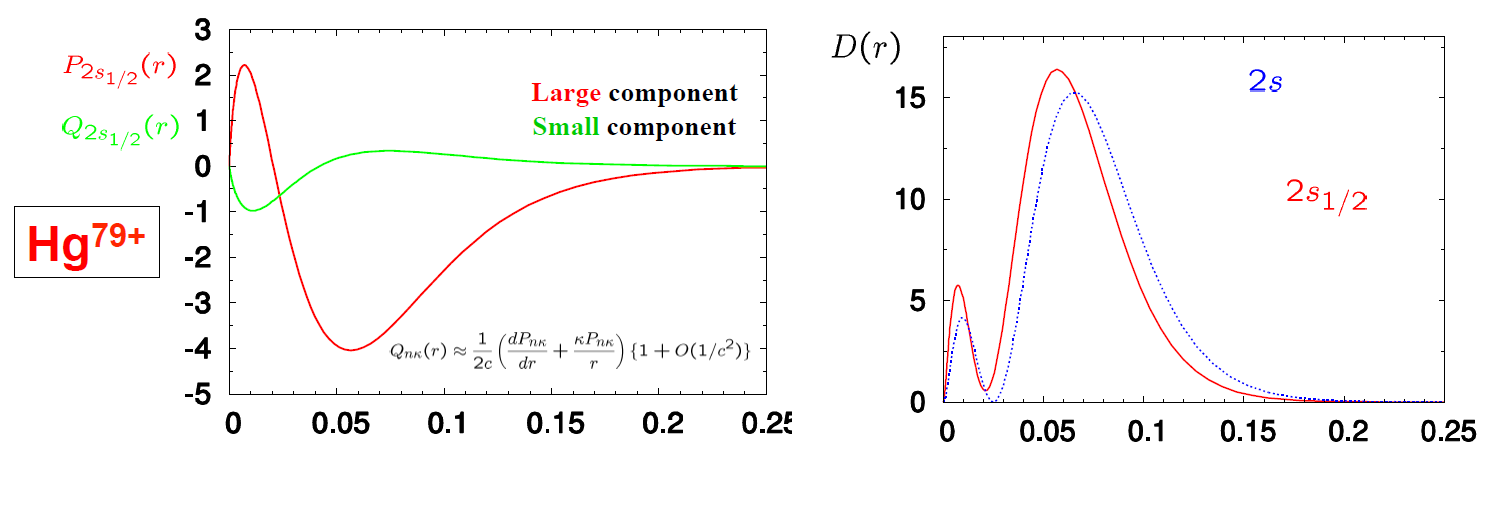
\includegraphics[scale=0.75]{ch1/image9.png}
	\captionof{figure}{ }
	\end{wrapfigure}
Soit $T_{max}$, l'énergie cinétique maximale qui peut être transférée dans une collision. 
Celle-ci est obtenue pour $p=0$, soit quand la particule cible est le plus proche possible
de la particule incidente. Nous ne sommes plus ici dans le cadre du précédent modèle (\textit{
soft collision}) mais ce n'est pas grave car seule une limite maximale est recherchée. L'image
ci-contre représente le système du laboratoire.\\

Dans le système du centre de masse (désigné par un \textit{prim})
\begin{equation}
v_{CM}=\frac{m_1v}{m_1+m_2},\qquad\qquad\qquad v'=v-v_{CM}
\end{equation}
Considérons une collision élastique avec uniquement un transfert d'énergie cinétique. L'intérêt
d'une telle collision dans le système du centre de masse est que seule la direction change : 
la vitesse et le module restent inchangés.
\begin{center}
	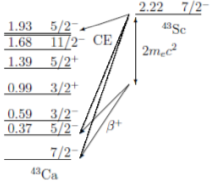
\includegraphics[scale=0.75]{ch1/image10.png}
	\captionof{figure}{ }
\end{center}
La situation correspondant à un maximum d'énergie transférée correspond à celle où la variation 
de la direction est la pus importante, soit quand tout change de sens. Dans le système du 
laboratoire, la vitesse maximale $v_{2,max}$ de la particule 2 s'écrit
\begin{equation}
v_{2,max}=\frac{2m_1v}{m_1+m_2}
\end{equation}
L'énergie maximale transférée vaut donc
\begin{equation}
T_{max}=\frac{m_2v_{2,max}^2}{2}=\gamma E
\end{equation}
où $\DS\gamma=\frac{4m_1m_2}{(m_1+m_2)^2} {\mbox{~~~~et~~~~}}E=\frac{m_1v^2}{2}$.\\

Ceci mène directement à deux implications 
\begin{enumerate}
\item Pour $m_1=m_2 \to \gamma=1$ ; l'énergie transférée peut valoir toute l'énergie de la particule
incidente
\item Pour $m_1\ll m_2$ ou l'inverse $\to \gamma$ petit
\end{enumerate}
Il en vient que\\

\cadre{\begin{itemize}
\item[$\bullet$] Un grand transfert d'énergie est possible pour l'interaction $e^-/e^-$
\item[$\bullet$] Un petit transfert d'énergie est possible pour l'interaction ion$/e^-$
\item[$\bullet$] Un petit transfert d'énergie est possible pour l'interaction $e^-/$ion
\item[$\bullet$] Un petit transfert d'énergie est possible pour l'interaction ion/ion
\end{itemize}
Notons que l'on parle de transfert possible et \textbf{pas} de probabilité.}

\newpage
\subsubsection{Détermination de l'énergie transférée minimale $T_{min}$}
Nous allons calculer $T_{min}$ dans le cas d'une collision avec un $e^-$ (il s'agit du cas
pratique le plus intéressant). Pour un électron isolé et libre, on trouve $T_{min}=0$. Or, 
la section efficace de stopping contient le logarithme du rapport $T_{max}/T_{min}$, il y 
aura divergence. Deux façon de lever la divergence existent
\begin{enumerate}
\item Considérer que les $e^-$ sont liés à une molécule ou à un atome
\item Considérer l'écrantage de l'interaction de Coulomb
\end{enumerate}
La première solution sera retenue?. Le plus simple est le modèle simple de Thompson où 
$T_{min}$ est l'énergie d'excitation la plus faible. Néanmoins, on s'intéressera ici 
au modèle de Bohr, plus proche du résultat quantique.\\

La vision de Bohr revient à voir la matière comme une collection d'oscillateurs harmonique 
classiques. En cas de choc lent $(2\pi/\omega_0\ll \tau$), l'oscillateur peut directement 
se remettre en place et le transfert d'énergie est négligeable (invariance adiabatique). 
L'orbite de l'électron n'est que provisoirement déformée, les états initiaux et finaux sont
identiques.\\

Si par contre le temps d'interaction est court par rapport à la période de l'oscillateur 
($\tau \ll 2\pi/\omega_0$), l'oscillateur reçoit une impulsion $F\times\tau$. C'est ce que
nous considérons ici. En utilisant l'expression du temps d'interaction, on trouve un ordre
pour $T_{min}$
\begin{equation}
\frac{2p}{v}\ll\frac{2\pi}{\omega_0} \Rightarrow p_{max}\sim\frac{v}{\omega_0}
 \Rightarrow T_{min}\sim\frac{2e_1^2e^2\omega_0^2}{mv^4}
\end{equation}
avec $\DS T\simeq \frac{2e_1^2e_2^2}{mv^2p^2}$ et $p_{max}$, le 
\textit{rayon adiabatique de Bohr}.\\

On peut alors, dans le modèle de Bohr (en reprenant les précedentes expressions), calculer 
la section efficace de stopping électronique comme il n'y a plus divergence \\

\cadre{\begin{equation}
S_e=\frac{4\pi Z_2 e_1^2e^2}{mv^2}L_e\quad\text{avec}\quad L_e=\ln\frac{Cmv^3}{|e_1e
|\omega_0}{\mbox{~~et~~}}C\simeq 1
\end{equation}
où $L=\frac{1}{2}\ln{\left(\frac{T_{max}}{T_{min}}\right)}$ et $C$, une correction introduite 
par Bohr que nous ne prendrons pas en compte.}


\subsubsection{Déviation angulaire maximale}
Soit $m_2\leq m_1$. Soit à gauche le référentiel du laboratoire et à droite, celui du centre de 
masse
\begin{center}
	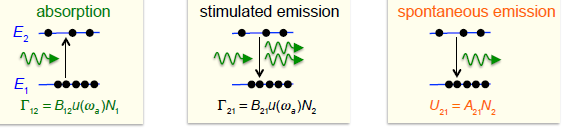
\includegraphics[scale=0.45]{ch1/image11.png}
	\captionof{figure}{ }
\end{center}
Dans le référentiel du centre de masse
\begin{equation}
v_{CM}=\frac{m_1}{m_1+m_2}v_{1i},\qquad\qquad\qquad v'=v-v_{CM}
\end{equation}
On en tire
\begin{equation}
v'_{1i}=v_{1i}-v_{CM}=\frac{m_2}{m_1+m_2}v_{1i}
\end{equation}
Comme nous avons une collision élastique dans le repère du centre de masse, seule la direction
est modifiée (et donc $v_{1f}'=v_{1i}'$)
\begin{equation}
v'_{1f}=\frac{m_2}{m_1+m_2}v_{1i}
\end{equation}

	\begin{wrapfigure}[8]{r}{5.5cm}
	\vspace{-5mm}
	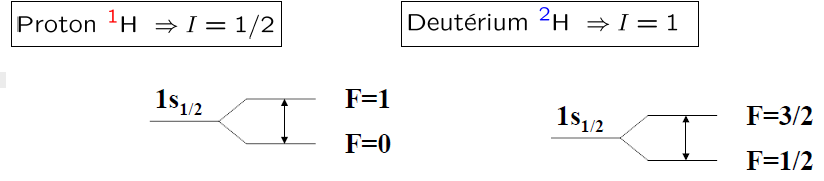
\includegraphics[scale=0.65]{ch1/image12.png}
	\captionof{figure}{ }
	\end{wrapfigure}

L'angle maximal $\theta_{max}$ est obtenu lorsqu'un angle droit est formé au niveau de la
circonférence du cercle. On choisit alors $v_{1f}'$ ($v_{CM}$) étant fixé de sorte à avoir
$\theta_{max}$. Après un peu de trigonométrie
\begin{equation}
\sin{\theta_{max}}=\frac{v'_{1f}}{v_{CM}}=\frac{m_2}{m_1}
\end{equation}
Si $m_2\geq m_1$, on trouve $\theta_{max}=\pi$. \\

En conclusion\\

\cadre{\begin{itemize}
\item[$\bullet$] Grandes déviations possibles ($\theta_{max}=\pi/2$) pour l'interaction $e^-/e^-$
\item[$\bullet$] Très grandes déviations possibles ($\theta_{max}=\pi$) pour l'interaction $e^-/$ion
\item[$\bullet$] Petites déviations pour l'interaction ion/$e^-$
\item[$\bullet$] Grandes déviations possibles (dépendant de $m_1$ et $m_2$) pour l'interaction ion/
ion
\end{itemize}}

\subsection{Conclusions à propos de ces considérations de base}
\subsubsection{Pour les ions incidents}
De façon générale les pertes électroniques dominent (petits transfert d'énergie et petites déviations
angulaires) et les pertes nucléaires (collisions noyaux) sont rares (se produisent pour un 
faible nombre de projectives mais de grand transferts d'énergies sont possibles ainsi que de 
grandes déviations angulaires). Ils ont une \textit{trajectoire rectilignes accompagnées de 
pertes d'énergie faibles et continues}.

\subsubsection{Pour les électrons incidents}
Les pertes électroniques dominent (mais cette fois grands transferts d'énergie et grandes déviations
angulaires possibles). On retrouve aussi des pertes nucléaires (petits transferts d'énergie mais
très grandes déviations angulaires possibles (possibilité de rétro-diffusion). Ils ont une 
\textit{trajectoire courbée accompagnée de grandes pertes d'énergie}.







%%%%%%%%%%%%%%%%%
% Bibliographie %
%%%%%%%%%%%%%%%%%
%\newpage
%\chapter{Bibliographie}
%\nocite{*}
%\printbibliography[heading=none]

%%%%%%%%%%%
% Annexes %
%%%%%%%%%%%
\appendix
%\input{annexes/annexe1.tex}


\end{document}
